\chapter{Summary}
\label{chap:summary}
This chapter provides a summary of the design concepts presented in chapter \ref{chap:conceptual-design} and the implementation of one of the concepts in chapter \ref{chap:implementation}.

\section{Design Concepts}
\label{sec:summary-concept}
In chapter \ref{chap:conceptual-design}, the rough and vague design of the first prototype discussed in section \ref{sec:prototype-design} was further refined over the course of two iterations.\\
The first design concept presented in section \ref{sec:design-1} describes a monolithic proxy application that builds on the basic initial design which makes extensive use of the pipes and filters design pattern for message routing. At its core it sends and receives packets (\emph{messages}) through gateways and (de-)serializes and transforms them through network stacks. It also features state-machines that allow implementation of complex logic of message (de-)serialization and transformation by allowing the binding of individual network stacks to states and triggering state transitions programmatically through the use of scripts. This results in a potentially deeply nested hierarchy of state-machines and network stacks.\\
The second design concept discussed in section \ref{sec:design-2} is an iteration of the monolithic design concept and describes a distributed proxy application that isolates (de-)serialization and transformation of messages from the internal proxy application logic. To decouple these low-level tasks from the high-level application logic of the proxy application, the concept introduces interfaces for remote units that provide access to specific features (i.e. (de-)serialization) and an interface for the central proxy application that allowed registering these remote units. Also, the nested hierarchy of state-machines and network stacks is flattened and organized centrally in a repository in the central proxy application.\\
Both concepts feature distinct advantages and disadvantages and are compared in section \ref{sec:design-comparison}.

\section{Implementation}
\label{sec:summary-implementation}
Chapter \ref{chap:implementation} shows an exemplaric implementation of the monolithic design concept discussed in section \ref{sec:design-1} under the working title \enquote{net-riot}. The monolithic design concept was chosen for implementation due to its proven core ideas and its comparatively high maturity. The second example scenario presented in section \ref{sec:example-scenarios} was used for reference because it features a nested communication stack and a corresponding testbed has already been implemented in section \ref{sec:prototype-testing}. For this implementation, Python is used because of its flexibility, low barrier of entry and rich package ecosystem.\\
Since the reference scenario makes use of the \ac{HTTP}, \ac{WS} and \ac{MQTT} protocols that used \ac{TCP} as an underlying transport protocol, \ac{TCP} gateways are implemented in net-riot as a \ac{MITM} interface that external devices such as \ac{IoT} devices and cloud servers can connect to. For \ac{HTTP} (de-)serialization, net-riot implements a custom encoder while for \ac{WS} and \ac{MQTT} existing libraries are used.\\
For representation of stacked communication protocols (such as \ac{MQTT} being transported via \ac{WS}), network stacks and state-machines were implemented: network stacks bundle a series of connected pipes that perform operations on messages, such as (de-)serializing and manipulating messages. State-machines allow selecting which network stacks to actively use by binding them to individual states. State-machines regularly evaluate their context and check whether states should be changed dependent on their registered transitions' rules. These ScriptRules execute scripts which can examine and manipulate the states' and state-machines' context information.\\
A central task left open for implementation by the design concept is the configuration of the proxy application for specific scenarios and the resulting dynamic instantiation and parametrisation of state-machines and network stacks. In net-riot, \ac{JSON} files and schemas were used for configuration specification and validation. Also, a recursive variance of the abstract factory design pattern was implemented for dynamic instantiation of objects defined in the configuration files. Figure \ref{fig:cloc} shows the output of the \enquote{cloc} utility program executed on net-riot's source code.\\
While net-riot implemented all components required by the scenario it was designed for, bugs in the implementation and challenging debugging ultimately lead to net-riot being unable to operate correctly in the testbed.

\begin{figure}[h]
    \centering
    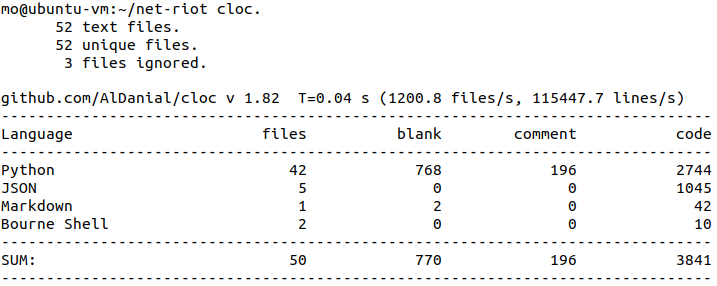
\includegraphics[width=12cm]{img/ch06/cloc2.png}
    \captionof{figure}{The lines of code in net-riot calculated by the \enquote{cloc} utility program.}
    \label{fig:cloc}
\end{figure}